\chapter{Background knowledge}
The section contains submodularity, the lower bound of GCB under the tree-structured graph, Prim and Dijkstra (PD) algorithm, and extended probability of detection (EPD).

\section{Submodularity}

The definition and illustration of submodularity are as follows:

\begin{definition}[Submodularity~\cite{nemhauser1978analysis}]
  Given a finite set $S=\{1,2,...,N\},$ a submodular function is a set function $F:2^N \rightarrow \mathbb{R}$ that satisfies the diminishing return property.
For every $S_A, S_B \subseteq S$ with $S_A \subseteq S_B$ and every $s \in S\setminus B,$
\begin{equation}
  \begin{aligned}
    F(S_A\cup s)-F(S_A) \geq F(S_B\cup s)-F(S_B)
  \end{aligned}
  \label{eq:submodular function}
\end{equation}
 holds.
\end{definition}

To illustrate the concept of submodularity, an example is shown in Fig.~\ref{fig:submodularity}. There are three ground sets ($S = \{1, 2, 3\}$).
$S_A=\{1\}$ and $S_B=\{1, 2\}$ represent the selected two sets, respectively. The set $S_B=\{1, 2\}$ means that the sensors are selected at location \textcircled{1} and \textcircled{2}.
$F(S_A)$ and $F(S_B)$ mean the coverage of sensor at location \textcircled{1} and \textcircled{1}\textcircled{2} (see Fig.~\ref{fig:submodularity}(a)(b)), respectively.
The submodular gain of $S_A$ and $S_B$ after adding a set $s = \{3\}$ is represented by the green dashing lines (see Fig.~\ref{fig:submodularity}(c)).
It is clear that the coverage function satisfies the diminishing return property (Eq.~\ref{eq:submodular function}). Alternatively, the objective function of maximizing coverage is submodular.
Greedy approaches can generate near-optimal solutions even if maximal coverage is NP-hard problem.

\begin{figure}[htbp]
 \begin{center}
\begin{subfigure}{.22\textwidth}
  \centering
  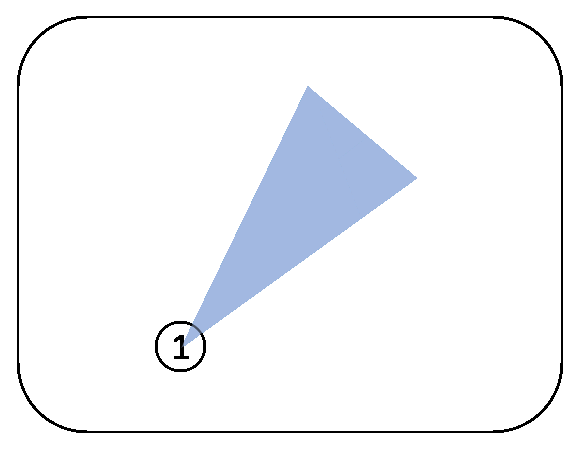
\includegraphics[width=1.0\linewidth]{sub6.eps}
  \caption{$F(S_A)$}
\end{subfigure}
\begin{subfigure}{.22\textwidth}
  \centering
  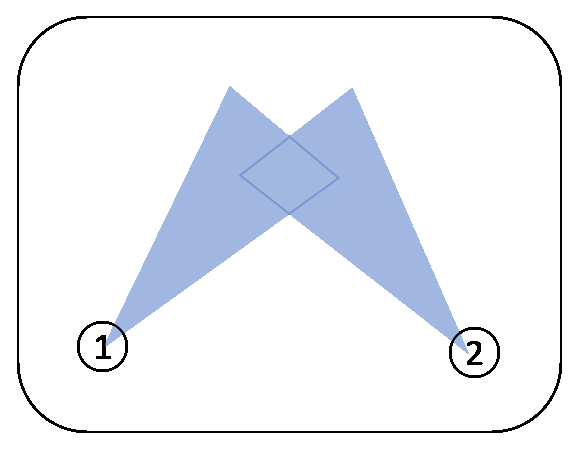
\includegraphics[width=1.0\linewidth]{sub7.eps}
  \caption{$F(S_B)$}
\end{subfigure}
\begin{subfigure}{.44\textwidth}
  \centering
  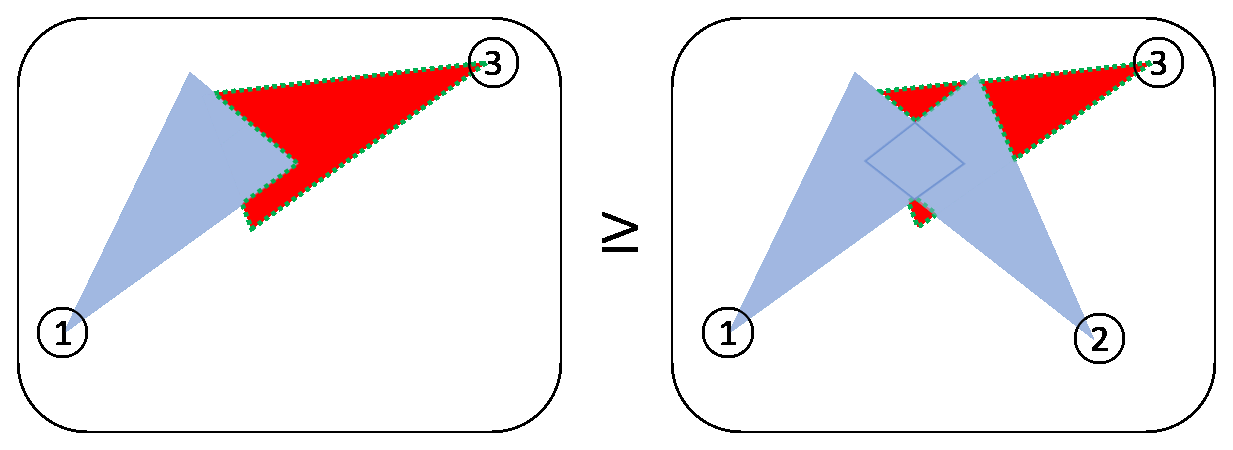
\includegraphics[width=1.0\linewidth]{sub5.eps}
  \caption{$F(S_A \cup s)-F(S_A)$ and $F(S_B \cup s)-F(S_B)$}
\end{subfigure}
\caption{Illustration of submodularity. The decimal number represents the selected sensor.
The colorful and white areas represent the covered and uncovered areas, respectively.
(a) $F(S_A)$ represents the covered area by $S_A,$ where $S_A = \{1\}.$ (b) $F(S_B)$ represents the covered area by $S_B,$ where $S_B = \{1, 2\}.$
(c) The green dash lines represent the submodular gain after adding $s,$ where $s = \{3\}.$ Left figure shows the $F(S_A\cup s) - F(S_A)$ and right figure shows that $F(S_B\cup s) - F(S_B).$}
\label{fig:submodularity}
 \end{center}
 \end{figure}

\section{Lower bound of GCB}
To further apply submodularity to routing constraints,
some definitions and the lower bound of GCB are introduced as follows:

\begin{definition}[Total curvature~\cite{conforti1984submodular}]
Given a finite set $S = \{1,2,...,N\},$
a monotone submodular function $f$, the total curvature of $f$ is defined as:

\begin{equation}
\kappa_f = 1 - \min_{s\in S:f(\{ s \}) > 0}\frac{f(S)-f(S \setminus\{ s \})}{f(\{ s \})}.
\label{eq:kappa}
\end{equation}

If the $\kappa_f = 0$, then $f$ is modular.
%Moreover, $\frac{1}{\alpha_f} \ge 1-\kappa_f \ge 0$ can be directly obtained from Def.~\ref{def:sub_ratio}~\cite{lin2023improvement}.
\label{def:kappa_f}
\end{definition}

\begin{definition}[The largest size of feasible solution $K_c$~\cite{zhang2016submodular}]
Given a ground set $S$ and cost function $c$, $K_c$ is defined as:

\begin{equation}
K_c = \max_{X\subseteq S}\{|X|\; | c(X) \le B\},
\end{equation}
where $B$ is budget.
\label{def:K_c}
\end{definition}

%\begin{theorem}[Lower bound of GCB~\cite{zhang2016submodular}]
%Given a submodular monotone set function $f$ and a monotone set function $c$,
%the GCB approach is to maximize f subject to the budget $B$.
%The GCB performance of a set X achieves
%\begin{equation}
%  f(X)\ge\frac{1}{2}(1-\frac{1}{e})f(\tilde{X}),
%\end{equation}
%where
%\begin{equation}
% \tilde{X} = arg\max _X\{
%f(X) | c(X)\le B\frac{ \alpha_{\hat{c}}(1 + \alpha_c^2 (K_c-1) (1-\kappa_c) )  }{ \psi(n) K_c }
%\}.
%\label{eq:noOPT}
%\end{equation}
%$c$ and $\hat{c}$ represent the cost function and the approximation cost function, respectively.
%The TSP solver is  $\psi(n)-$approximation (i.e. $c(X) \le \hat{c}(X) \le \psi(n)c(X),$ and $\psi(n) \ge 1$).
%
%\label{thm:GCB}
%\end{theorem}

\begin{theorem}[Lower bound of GCB under the tree-structured graph~\cite{lin2023improvement}]
Given a submodular monotone set function $f$ and a tree-structured graph cost function $c$,
the GCB approach is to maximize f subject to the budget $B$.
The performance of a set X achieves
\begin{equation}
  f(X)\ge\frac{1}{2}(1-\frac{1}{e})f(\overline{X}),
\end{equation}
where
\begin{equation}
 \overline{X} = \arg\max _X\{
f(X) | c(X)\le B(1-\kappa_c + \frac{\kappa_c}{K_c})
\}.
\label{eq:OPT_lin}
\end{equation}

\label{thm:GCB_lin}
\end{theorem}

\section{Prim and Dijkstra (PD) algorithm}

Minimum spanning tree is to minimize the total weight (TW) in a weighted undirected graph.
Prim's algorithm is a well-known greedy algorithm to find a minimum spanning tree for a weighted undirected graph~\cite{prim1957shortest}.
%The idea is to maintain two sets of vertices,
%the vertices in the MST and the vertices not in the MST.

Dijkstra algorithm is a well-known algorithm to find the shortest path between source node and terminal node in an undirected weighted graph.
Dijkstra algorithm is adopted for SPT to find the source point between the other nodes in graph.
To combine Prim and Dijkstra algorithms, the objective function is proposed as follows:

\begin{definition}[The objective function of Prim and Dijkstra algorithm~\cite{alpert1993direct}]
The $v_i$ and $v_j$ of Prim and Dijkstra algorithm are chosen to minimize
\begin{equation}
  \begin{aligned}
    (\alpha\cdot l_i)+d_{ij} \; s.t. \; v_j\in T, v_i \in V - T,
  \end{aligned}
  \label{eq:PD_obj}
\end{equation}
where $\alpha\in[0, 1]$ is a tuning parameter, $l_i$ is the length from source (start point) to node $v_i$, $d_{ij}$ is the distance between $v_i$ and $v_j$, $V$ is all vertices in graph and $T$ is current growing tree.
\end{definition}

Prim-Dijkstra (\emph{PD}) algorithm~\cite{alpert1993direct} can generate different types of spanning trees.
If $\alpha = 0$, PD algorithm is Prim algorithm; if $\alpha = 1$, PD algorithm is Dijkstra algorithm.
As Fig.~\ref{fig:PD_intro}(a) shows, there are six subgoals on this map.
As Fig.~\ref{fig:PD_intro}(b) shows, the Prim algorithm generates the minimum spanning tree (MST).
As Fig.~\ref{fig:PD_intro}(c) shows, the Dijkstra algorithm on this map generates the shortest path tree.
In the \emph{PD} algorithm, different parameters generate different spanning trees.
%For example,
%if $\alpha = 0$, PL = $13.969$ and TW = $5.393$ in Fig.~\ref{fig:PD_intro} (b).
%If $\alpha = 1$, PL = $7.658$ and TW = $7.658$ in Fig.~\ref{fig:PD_intro} (c).
%If $\alpha = 0.5$, PL = $8.119$ and TW = $6.726$ in Fig.~\ref{fig:PD_intro} (d).
%(c), these trees are edge cases generated by the \emph{PD} algorithm.
%{\color{olive}As Fig.~\ref{fig:PD_intro}(d) shows, the \emph{PD} algorithm in this map generates various spanning trees.
%This research analyzes the performances of different types of spanning trees.

%The inputs are an undirected graph ($G$), the source ($s$).
%The output is the spanning tree.
%Line $1$ is to build $Q$ (vertices in $G$).
%Line $2-3$ is initializing.
%Line $5$ is to find the distance connecting $v_q$ and $v_k$, where $v_q$ belongs to the current growing tree ($S$), and $v_k$ does not belong to the current growing tree {\color{olive}of the tree}.
%Line $6$ is to find the path length from {\color{olive}the} source vertex to $v_q$ along the current growing tree ($S$).
%Line $7$ is to trade off Prim algorithm and Dijkstra algorithm.
%{\color{olive}Line $8-9$ is to update current tree and spanning tree.}
%{\color{red} (How about plotting a figure to explain it. Here is background knowledge. )}


%The PD algorithm is to trade off between MST and SPT.
%The $\alpha$ is a weighting parameter that allows to span the entire tradeoff range.
%When $\alpha = 0$, the PD algorithm results in generating MST.
%When $\alpha = 1$, the PD algorithm results in generating SPT.



%\begin{algorithm}[ht]	
%	\KwIn{\\
%$G = (V, E, w)$: undirected graph \\
%$s$: the start point
%}
%\KwOut{$S$: spanning tree}
%\Parameter{$\alpha$ (between $0$ and $1$)}
%	\caption{Prim and Dijkstra algorithm}
%	\begin{algorithmic}[1]
%    \State {$Q = V$ \#all of vertices in $G$}
%    \State {$Q = Q \setminus \{s\}$}
%    \State {$S = \phi$}
%    \WHILE {$Q \neq \phi$}
%        \State {let $d_{qk}$ be the cost edge such that $q \in Q$ and $k \in V \setminus Q$}
%        \State {$pl_q$ is distance from source to $v_q$}
%        \State {minimize ($\alpha\times pl_i+d_{iu}$) where $i\in Q,$ $u\in V\setminus Q$}
%        \State {$Q = Q \setminus \{i\}$}
%        \State {$S = S \cup (u, i)$}
%    \ENDWHILE	
%    \end{algorithmic}	
%	\label{al:PD}
%\end{algorithm}

\begin{figure}[htbp]
 \begin{center}
\begin{subfigure}{.22\textwidth}
  \centering
  \includegraphics[width=1.0\linewidth]{pt.jpg}
  \caption{The complete graph}
\end{subfigure}
\begin{subfigure}{.22\textwidth}
  \centering
  \includegraphics[width=1.0\linewidth]{toy_alpha_00.jpg}
  \caption{MST ($\alpha=0$)}
\end{subfigure}
\begin{subfigure}{.22\textwidth}
  \centering
  \includegraphics[width=1.0\linewidth]{toy_alpha_10.jpg}
  \caption{SPT ($\alpha=1$)}
\end{subfigure}
\begin{subfigure}{.22\textwidth}
  \centering
  \includegraphics[width=1.0\linewidth]{toy_alpha_05.jpg}
  \caption{Tree $(\alpha=0.5)$}
\end{subfigure}
\caption{Illustration of the \emph{PD} algorithm. (a) The complete graph.
The blue points, blue edges and decimal numbers represent subgoals, paths and the index of subgoals, respectively.
(b) Minimum spanning tree (MST).
(c) Shortest path tree (SPT).
(d) The tree between MST and SPT. Tuning the $\alpha$ parameter generates different spanning trees.
}
\label{fig:PD_intro}
 \end{center}
 \end{figure}

\section{Extended probability of detection (EPD)}


IPP problems can be formulated as POMDP problems~\cite{kadane1977optimal}, which are NP-hard. Hence, probability of detection model is proposed.
However, the assumptions of probability of detection are not realistic, i.e., the agent only moves to neighbor cells, and the sensor has no overlapping covearge. The extended probability of detection (EPD) was proposed~\cite{tseng2016learning} to apply to real world.
The definition of EPD is as follows:

\begin{definition}[Extended probability of detection (EPD)~\cite{tseng2016learning}]
The agent gets the information $z$.
The assumptions of EPD are as follows:\\
(i) There is no target detection ($z = 1$) along the path.\\
(ii) The sensing overlapping is available.\\
(iii) The agent could move to any subgoals.\\
The equation of the cumulative EPD is defined as
\begin{equation}\label{eq:cepd}
  f_p(S_g) = \sum_{i=1}^{T}P(S_{g,i})\cdot g
\end{equation}
, where $f_p$ is the cumulative EPD along the path, $g$ is glimpse function and $P(S_{g,i})$ is the probability of covered cells at the i-th subgoal. The value of glimpse function can be calculated from the confusion table.

\end{definition}

As Fig.~\ref{fig:EPD_z} shows, the agent's sensing area is not fitting in its local cell.
Due to the availability of sensing overlap, the probability of sensing area is recomputed.
The assumption is that the agent moves along the path without any detections ($z=0$).
Finally, the agent can navigate to any subgoals instead of neighborhood areas.


%\begin{figure}[t!]
% \begin{center}
%  \centering
%  \includegraphics[width=0.5\linewidth]{EPD.jpg}
%\caption{Illustration of Extended probability of detection. The white and green areas represent low probability and high probability, respectively.  {\color{red} (you should plot the branches (z=1, z=0)?)}}
%\label{fig:EPD}
% \end{center}
% \end{figure}

\begin{figure}[htbp]
 \begin{center}
  \centering
  \includegraphics[width=0.5\linewidth]{EPD_z.jpg}
\caption{Illustration of no detection. In the PD assumption, the agent assumes there is no detection of a target along a path.}
\label{fig:EPD_z}
 \end{center}
 \end{figure} 